% 生成最终的图象时把第一个文档类取消注释即可
\documentclass[10pt]{standalone}
% \documentclass[10pt]{article}
% 1.必须添加varwidth选项,不然就会报错
% \PassOptionsToPackage{quiet}{fontspec}
% \usepackage{ctex}
% 必须要保证绘图的纸张足够的大
% \usepackage[a4paper, left=2.5cm, right=2.5cm, top=2.5cm, bottom=2.5cm]{geometry}
\usepackage{xifthen}
\usepackage{xfp}
\usepackage{xcolor}
\usepackage{pgfplots}
\usepackage{pgfplotstable}
\pgfplotsset{compat=1.16}
% 2.引用的tikz库
\usetikzlibrary {matrix, chains, trees, decorations}
\usetikzlibrary {arrows.meta, automata,positioning}
\usetikzlibrary {decorations.pathmorphing, calc}
\usetikzlibrary {calligraphy}
\usetikzlibrary {backgrounds, mindmap,shadows}
\usetikzlibrary {patterns, quotes, 3d, shadows}
\usetikzlibrary {graphs, fadings, scopes}
\usetikzlibrary {arrows, shapes.geometric}
\usepgflibrary {shadings}


\begin{document}
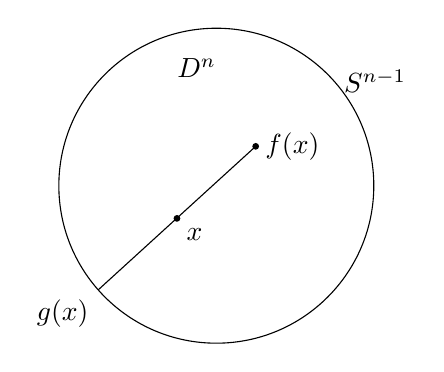
\begin{tikzpicture}
  \draw (0, 0) circle (2cm);
  \node at (-.25, 1.5) {$D^n$};
  \node[right] at (1.5, \fpeval{sqrt(4-1.5^2)}) {$S^{n-1}$};
  \draw (.5, .5) -- (-1.5, \fpeval{-sqrt(4-1.5^2)}) node[below left] {$g(x)$};
  \filldraw (.5, .5)node[right]{$f(x)$} circle (1pt);
  \filldraw (-.5, -.415)node[below right]{$x$} circle (1pt);
\end{tikzpicture}
\end{document}